\documentclass[letterpaper, 10 pt, conference]{ieeeconf}  % Comment this line out if you need a4paper
%\documentclass[a4paper, 10pt, conference]{ieeeconf}      % Use this line for a4 paper

\IEEEoverridecommandlockouts                              % This command is only needed if 
                                                          % you want to use the \thanks command

\overrideIEEEmargins                                      % Needed to meet printer requirements.

% See the \addtolength command later in the file to balance the column lengths
% on the last page of the document

\usepackage[dvipdfmx]{graphicx}
\graphicspath{{figs/}}
\usepackage{amsmath}
\usepackage{amssymb}
%\usepackage{algorithm}
%\usepackage{algpseudocode}
%\usepackage{times}
\usepackage{bm}
%\usepackage{here}

\newcommand{\figref}[1]{Fig. \ref{figure:#1}}
\newcommand{\tabref}[1]{Table \ref{table:#1}}
\newcommand{\equref}[1]{Eq. \ref{eq:#1}}
\newcommand{\argmax}{\operatornamewithlimits{argmax}}
\newcommand{\argmin}{\operatornamewithlimits{argmin}}

%\setcounter{topnumber}{100}
%\setcounter{bottomnumber}{100}
%\setcounter{totalnumber}{100}
%\renewcommand{\textfraction}{0.0}
%\renewcommand{\topfraction}{1.0}


\title{\LARGE \bf
  %Form Optimization Control for Multiple Objects Transportation by Transformable Multirotor with Two-dimensional Multilinks
  %Form Optimization Control for Multiple Objects Transportation by Multilinked Multirotor with Internal Communication System
  Multilinked Multirotor with Internal Communication System for Multiple Objects Transportation based on Form Optimization Control
}


\author{Tomoki Anzai$^{1}$, Moju Zhao$^{1}$, Xiangyu Chen$^{1}$, Fan Shi$^{1}$, Koji Kawasaki$^{1}$, Kei Okada$^{1}$, Masayuki Inaba$^{1}$% <-this % stops a space
%\thanks{*This work was not supported by any organization}% <-this % stops a space
\thanks{$^{1}$T. Anzai, M. Zhao, X. Chen, F. Shi, K. Kawasaki, K. Okada and M. Inaba are with Department of Mechano-Informatics, The University of Tokyo, 7-3-1 Hongo, Bunkyo-Ku, Tokyo 113-8656, Japan
       {\tt\small anzai at jsk.t.u-tokyo.ac.jp}}%
%\thanks{$^{2}$Bernard D. Researcheris with the Department of Electrical Engineering, Wright State University,
%        Dayton, OH 45435, USA
%        {\tt\small b.d.researcher@ieee.org}}%
}


\begin{document}

\maketitle
\thispagestyle{empty}
\pagestyle{empty}

\begin{abstract}
\input src/abst.tex
\end{abstract}

\input src/intro.tex
\input src/approaches.tex
\input src/flight_control.tex
\input src/system.tex
\input src/optimization.tex
\input src/experiments.tex
\input src/conclusion.tex

\addtolength{\textheight}{-12cm}   % This command serves to balance the column lengths
                                  % on the last page of the document manually. It shortens
                                  % the textheight of the last page by a suitable amount.
                                  % This command does not take effect until the next page
                                  % so it should come on the page before the last. Make
                                  % sure that you do not shorten the textheight too much.

%\input src/appendix.tex
%\input src/acknowledge.tex


\begin{figure}[h]                                                                       
  \begin{center}                                                                        
    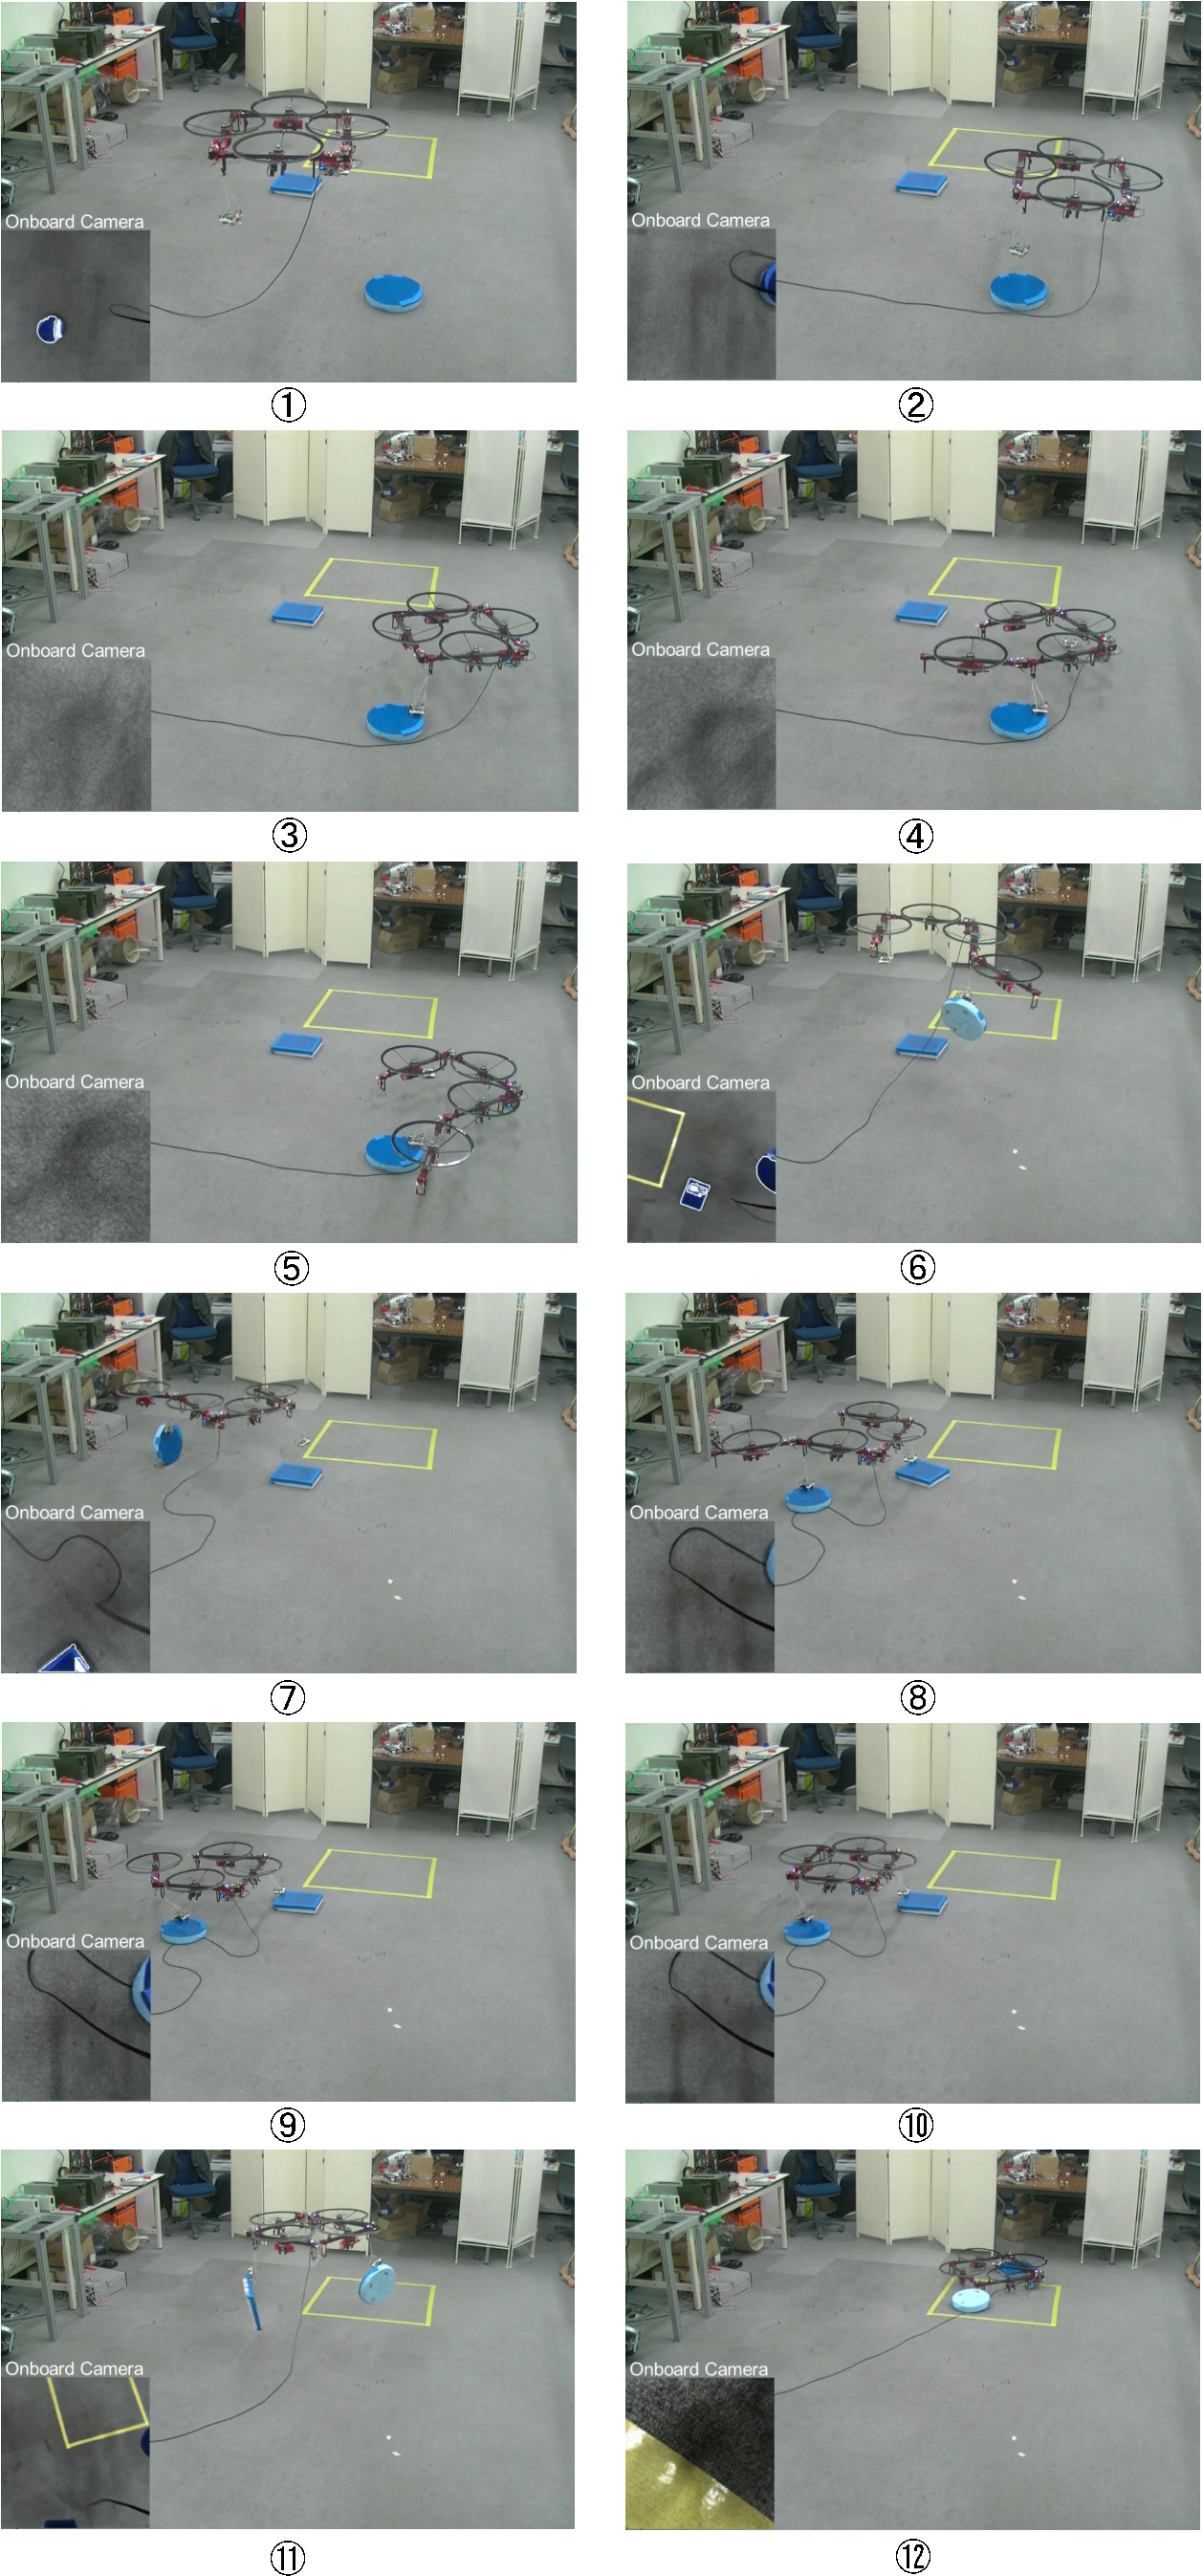
\includegraphics[width=1.0\columnwidth]{figs/experiment.pdf}                        
  \end{center}                                                                          
  \caption{Experiment of multiple objects transportation: two ferrous objects are grasped and transported by the transformable aerial robot. Lower left: the result of detection by onboard camera. \label{figure:experiment}}          
\end{figure}

%\bibliographystyle{junsrt}
%\bibliography{main}
\input ./main_saved.bbl     

\end{document}
